\documentclass[letterpaper,12pt]{article}

% @@@@@@@@@@@@@@@@@@@@@@@@@@@@@@@@@@@@@@@@@@@@@@@@@@@@@@@@@@@@>
% VALORES A MODIFICAR POR USTED:
% @@@@@@@@@@@@@@@@@@@@@@@@@@@@@@@@@@@@@@@@@@@@@@@@@@@@@@@@@@@@>

% NOTE: Leer nota en el README sobre la font.

\newcommand{\titulo}{Procedimiento ETL sobre los registros de actividad de los telescopios UT del Observatorio Paranal para la
generación de datasets del sistema de óptica activa de los espejos M1.}
\newcommand{\ciudad}{Santiago} % e.g. Valparaíso
% TODO: Consultar el formato de los nombres:
\newcommand{\nombrealumno}{Ignacio Ortiz Valdebenito}
\newcommand{\nombreprofesor}{Pedro Toledo Correa}
\newcommand{\nombrecorreferente}{Jose Luis Martí Lara}
% Mes y año del examen
\newcommand{\mesexamen}{Diciembre}
\newcommand{\anioexamen}{20XX}
% Dedicatoria y agradecimientos
\newcommand{\dedicatoria}{
Considerando lo importancia de este trabajo para los alumnos, este apartado es para que el autor entregue palabras personales para dedicar este documento. La extensión puede ser de máximo una hoja y se deben mantener este formato, tipo y tamaño de letra.
}
\newcommand{\agradecimientos}{
Considerando la importancia de este trabajo para los alumnos, este apartado se podrá incluir en el caso de que el autor desee agradecer a las personas que facilitaron alguna ayuda relevante en su trabajo para la realización de este documento. La extensión puede ser de máximo una hoja y se deben mantener este formato, tipo y tamaño de letra.
}
\newcommand{\resumen}{
El resumen y las palabras clave no deben superar la mitad de la página, donde debe precisarse brevemente: 1) lo que el autor ha hecho, 2) cómo lo hizo (sólo si es importante detallarlo), 3) los resultados principales, 4) la relevancia de los resultados. El resumen es una representación abreviada, pero comprensiva de la memoria y debe informar sobre el objetivo, la metodología y los resultados del trabajo realizado.
}
\newcommand{\resumeningles}{
Corresponde a la traducción al idioma inglés del Resumen anterior. Sujeto a la misma regla de extensión del Resumen.
}
\newcommand{\palabrasclave}{
Cinco es el máximo de palabras clave para describir los temas tratados en la memoria, ponerlas separadas por punto y comas.
}
\newcommand{\palabrasclaveingles}{
Corresponde a la traducción al idioma inglés de Palabras Clave anteriores.
}
% @@@@@@@@@@@@@@@@@@@@@@@@@@@@@@@@@@@@@@@@@@@@@@@@@@@@@@@@@@@@>

% Paquete para importar imágenes
\usepackage{graphicx}
% Directorio de las imágenes
\graphicspath{ {figures/} }

% Idioma y fuentes
\usepackage[spanish,es-tabla]{babel}
\usepackage[T1]{fontenc}

\usepackage{fontspec}
% Los siguientes comandos fueron sugeridos por @anibalbastiass (ver issue#5)
% para contar con Carlito en cursiva y negrita.
\setmainfont{Carlito}[BoldFont={* Bold}]
\setmainfont{Carlito}[ItalicFont={* Italic}]

% Paquete para definir cualquier tamaño de font
\usepackage{anyfontsize}

% Paquete para la bibliografia
\usepackage{cite}

% Settear font
\setmainfont{Carlito}

% Tamaño de la página y márgenes
\usepackage[letterpaper,top=2.5cm,bottom=3cm,left=3cm,right=3cm,marginparwidth=1.75cm]{geometry}

% Habilita los comentarios al margen, comentar para versión final
% Para desabilitar los comentarios y cambios de margen comentar la siguiente linea
%\newcommand{\comentado}{}
% Paquete para comentarios
%\usepackage{sidenotes}
% Package para color en los comentarios
%\usepackage{xcolor}
% Comando para habilitar y desabilitar comentarios al margen

%\newcommand{\comentario}[1]{
%	\ifdefined\comentado
%		\sidenote{\textcolor{red}{#1}}
%	\fi
%}

% Determinar interlineado:
\renewcommand{\baselinestretch}{1.0}

% Eliminar sangrías:
\setlength{\parindent}{0cm}

% Paquete para definir los formatos de los títulos
\usepackage[explicit]{titlesec}

\titleformat{name=\section}[block]{\fontsize{16}{24}\selectfont\bfseries}{}{0pt}{#1}
\titleformat{name=\section,numberless}[block]{\fontsize{16}{24}\selectfont\bfseries}{}{0pt}{#1}
\titlespacing*{name=\section}{0pt}{0pt}{0.5cm}
\titlespacing*{name=\section,numberless}{0pt}{0pt}{0.5cm}

% Separación entre parrafos
\setlength{\parskip}{0.4cm}

% Paquetes de utilidad general
\usepackage{amsmath}
\usepackage{graphicx}
\usepackage{float}
\usepackage[colorlinks=true, allcolors=blue]{hyperref}

% Formato de las tablas de contenido
\usepackage{tocbasic}

%% Originalmente se usaba tocstyle en vez de tocbasic.
%% Si se quiere usar, descomentar:
% \usepackage[tocflat]{tocstyle}
% \usetocstyle{allwithdot}
%% tocstyle.sty se obtener de https://github.com/firemodels/fds/blob/master/Manuals/LaTeX_Style_Files/tocstyle.sty

% Para obtener el número de la última página
\usepackage{lastpage}

% Header y footer
\usepackage{fancyhdr}
\fancypagestyle{portada}{
    \lhead{}
    \chead{}
    \rhead{}
    \lfoot{}
    \cfoot{\fontsize{10}{12}\selectfont \thepage}
    \rfoot{}
    \renewcommand{\headrulewidth}{0pt}
}
\fancypagestyle{intermedio}{
    \lhead{}
    \chead{\fontsize{10}{12}\selectfont\MakeUppercase{\titulo}}
    \rhead{}
    \lfoot{}
    \cfoot{\fontsize{10}{12}\selectfont Página \textbf{\thepage}\ de \textbf{\pageref{LastPage}}}
    \rfoot{}
    \renewcommand{\headrulewidth}{1pt}
}

% Comandos para secciones
\newcommand{\secnumbersection}[1]{
\addtocounter{section}{1}
\phantomsection
\section*{CAPÍTULO \thesection \texorpdfstring{\\}\ #1}
\addcontentsline{toc}{section}{CAPÍTULO \thesection : #1}
\setcounter{subsection}{0}
}
\newcommand{\secnumberlesssection}[1]{
\section*{#1}
\phantomsection
\addcontentsline{toc}{section}{#1}
\setcounter{subsection}{0}
}

% Nombres
\addto\captionsspanish{\renewcommand{\contentsname}{ÍNDICE DE CONTENIDOS}}
\addto\captionsspanish{\renewcommand{\listfigurename}{ÍNDICE DE FIGURAS}}
\addto\captionsspanish{\renewcommand{\listtablename}{ÍNDICE DE TABLAS}}
\makeatletter
\renewenvironment{thebibliography}[1]
     {\secnumberlesssection{REFERENCIAS BIBLIOGRÁFICAS}
      \@mkboth{\MakeUppercase\bibname}{\MakeUppercase\bibname}%
      \list{\@biblabel{\@arabic\c@enumiv}}%
           {\settowidth\labelwidth{\@biblabel{#1}}%
            \leftmargin\labelwidth
            \advance\leftmargin\labelsep
            \@openbib@code
            \usecounter{enumiv}%
            \let\p@enumiv\@empty
            \renewcommand\theenumiv{\@arabic\c@enumiv}}%
      \sloppy
      \clubpenalty4000
      \@clubpenalty \clubpenalty
      \widowpenalty4000%
      \sfcode`\.\@m}
     {\def\@noitemerr
       {\@latex@warning{Empty `thebibliography' environment}}%
      \endlist}
\makeatother

% Personalizar Tabla de Contenidos

\usepackage{tocloft}
\renewcommand{\cftsecfont}{\fontsize{12}{14}\selectfont\fontspec{Carlito}}
\renewcommand{\cftsubsecfont}{\fontsize{12}{14}\selectfont\fontspec{Carlito}}
\renewcommand{\cftsubsubsecfont}{\fontsize{12}{14}\selectfont\fontspec{Carlito}}

\renewcommand\cftfigfont{\fontsize{12}{14}\selectfont\fontspec{Carlito}}

% Links sin color
\usepackage{hyperref}
\hypersetup{colorlinks = false}

% Comando para secciónes sin enumeración
% (sugerido por @anibalbastiass https://github.com/autopawn/tex-thesis-template/issues/5#issuecomment-916106128)
\newcommand{\secnumberlesssubsection}[1]{
\subsection*{#1}
\phantomsection
\addcontentsline{toc}{subsection}{#1}
\setcounter{subsection}{0}
}
% Forma de uso:
% \secnumberlesssubsection{"Sub seccion sin enumeración"}

% @@@@@@@@@@@@@@@@@@@@@@@@@@@@@@@@@@@@@@@@@@@@@@@@@@@@@@@@@@@@>
\begin{document}
\sloppy % Para evitar que referencias se escapen de los márgenes.

\pagestyle{portada}
\pagenumbering{roman}
% NOTE: Este archivo contiene la portada, la dedicatoria, los agradecimientos y el resumen.
% __NO ES NECESARIO MODIFICAR ESTE ARCHIVO__, esas se modifican con los comandos que aparecen en main.tex
%@@@@@@@@@@@@@@@@@@@@@@@@@@@@@@@@@@@@@@@@@@@@@@@@@@@@@@@@@@@@@@
\begin{titlepage}
\begin{center}
\noindent
{\fontsize{18}{22}\selectfont UNIVERSIDAD TÉCNICA FEDERICO SANTA MARÍA \\}
{\fontsize{16}{19}\selectfont DEPARTAMENTO DE INFORMÁTICA \\}
{\fontsize{16}{19}\selectfont \MakeUppercase{\ciudad}\ - CHILE \\}
\vspace{1.5cm}

\includegraphics[width=4.41cm,height=3.34cm]{logo/logo.jpg} \\
\vspace{1.5cm}
{\fontsize{20}{24}\selectfont ``\MakeUppercase{\titulo}'' \\}
\vfill
{\fontsize{16}{19}\selectfont \MakeUppercase{\nombrealumno} \\}
\vfill
{\fontsize{16}{19}\selectfont MEMORIA PARA OPTAR AL TÍTULO DE \\}
{\fontsize{16}{19}\selectfont INGENIERO CIVIL EN INFORMÁTICA \\}
\vspace{1.5cm}
{\fontsize{14}{17}\selectfont Profesor Guía: \nombreprofesor \\}
{\fontsize{14}{17}\selectfont Profesor Correferente: \nombrecorreferente \\}
\vspace{2.5cm}
{\fontsize{14}{17}\selectfont \mesexamen\ - \anioexamen \\}
\end{center}
\end{titlepage}

%@@@@@@@@@@@@@@@@@@@@@@@@@@@@@@@@@@@@@@@@@@@@@@@@@@@@@@@@@@@@@@
%\newpage
%\setcounter{page}{2}
%\
%\vfill
%\vfill
%\begin{flushright}
%\noindent {\fontsize{16}{19}\selectfont \textbf{DEDICATORIA} \\}
%\end{flushright}
%\begin{flushright}
%\noindent \dedicatoria
%\end{flushright}
%\vfill
%@@@@@@@@@@@@@@@@@@@@@@@@@@@@@@@@@@@@@@@@@@@@@@@@@@@@@@@@@@@@@@
%\newpage
%\begin{center}
%\noindent {\fontsize{16}{19}\selectfont \textbf{AGRADECIMIENTOS} \\}
%\end{center}
%\noindent \agradecimientos
%\vfill
%@@@@@@@@@@@@@@@@@@@@@@@@@@@@@@@@@@@@@@@@@@@@@@@@@@@@@@@@@@@@@@
%\newpage
%\secnumberlesssection{RESUMEN}
%\vspace{0.3cm}
%\noindent \textbf{Resumen---}\resumen \ \\
%\vspace{0.3cm} \\
%\noindent \textbf{Palabras Clave---}\palabrasclave \ \\
% @@@@@
%\vspace{1.2cm} \\
% @@@@@
%\noindent {\fontsize{16}{19}\selectfont \textbf{ABSTRACT}}
%\vspace{1.2cm} \\
%\secnumberlesssection{ABSTRACT}
%\vspace{0.3cm}
%\noindent \textbf{\emph{Abstract}---}\resumeningles \ \\
%\vspace{0.3cm} \\
%\noindent \textbf{\emph{Keywords}---}\palabrasclaveingles \ \\
%@@@@@@@@@@@@@@@@@@@@@@@@@@@@@@@@@@@@@@@@@@@@@@@@@@@@@@@@@@@@@@


\newpage
\secnumberlesssection{GLOSARIO}

Aquí se deben colocar las siglas mencionadas en el trabajo y su explicación, por orden alfabético. Por ejemplo: \\

{\setlength{\parskip}{0cm} % Para evitar saltar entre cada elemento nombrado.
%Colocar aquí siglas:
DI: Departamento de Informática.

UTFSM: Universidad Técnica Federico Santa María.
}


%Índice de contenidos:
%\newpage
%\thispagestyle{portada}
%\tableofcontents

%Índice de figuras:
%\newpage
%\thispagestyle{portada}
%\phantomsection
%\addcontentsline{toc}{section}{ÍNDICE DE FIGURAS}
%\listoffigures
%\phantomsection
%\addcontentsline{toc}{section}{ÍNDICE DE TABLAS}
%\listoftables

\newpage
\pagestyle{intermedio}
\pagenumbering{arabic}

% Ajustes de margen para comentarios al margen
%\ifdefined\comentado
%  \newgeometry{right=\dimexpr 10.795cm, marginparwidth=\dimexpr 7.795cm-5pt}
%\fi

%\secnumberlesssection{INTRODUCCIÓN}

Debe proporcionar a un lector los antecedentes suficientes para poder contextualizar en general la situación tratada, a través de una descripción breve del área de trabajo y del tema particular abordado, siendo bueno especificar la naturaleza y alcance del problema; así como describir el tipo de propuesta de solución que se realiza, esbozar la metodología a ser empleada e introducir a la estructura del documento mismo de la memoria.

En el fondo, que el lector al leer la Introducción pueda tener una síntesis de cómo fue desarrollada la memoria, a diferencia del Resumen dónde se explicita más qué se hizo, no cómo se hizo.

%\newpage
\secnumbersection{DEFINICIÓN DEL PROBLEMA}

\subsection{DEFINICIÓN}

Los datos producidos por la Óptica Activa del telescopio VLT en Paranal poseen un tamaño y un formato tal que los vuelven
inutilizables para su uso en análisis y ciencia de datos externo.

\subsection{CONTEXTO}

El Telescopio Muy Grande (VLT por sus siglas en inglés) es uno de los telescopios ópticos más avanzados del mundo, compuesto de 4 Telescopios Unitarios (UT por sus siglas en inglés) y 3 Telescopios Auxiliares (AT por sus siglas en inglés).
Perteneciente al Observatorio Europeo Austral (ESO por sus siglas en inglés), el telescopio se ubica en el Cerro Paranal en el Norte de Chile, y se dedica principalmente a la búsqueda y estudio de galaxias y otras estructuras interestelares (1).
Para cumplir con estos objetivos, el telescopio debe cumplir con altos estándares tecnológicos, de entre los cuales se destaca la necesidad de una alta resolución angular y una alta calidad de imagen (1). Dicha responsabilidad recae principalmente en los UTs.

\\

Los UTs son telescopios de 8.2 metros que pueden trabajar solos o en conjunto, donde en este último modo alcanza el poder de colecta de luz de un solo telescopio de 16 metros.
Cada UT esta sobre una montura altazimutal, y el tubo del telescopio consiste de una estrucutra de acero apoyando en su parte inferior al Espejo Primario (M1 en inglés), y en su parte superior a la Unidad M2, la cuál corresponde al Espejo Secundario (M2 en inglés) con un mecanismo electromecánico que sujeta y controla la posición
del M2 más los respectivos circuitos electrónicos (2).

Bajo M1 se encuentran 150 actuadores de fuerza axiales, los cuales dan a M1 una determinada forma óptima según el patrón de fuerza presentado en los actuadores (1).
La forma en que cada telescopio captura las imagenes es la siguiente; primero se captura los rayos de luz estelares con el M1, y se concentra entre el M1 y el M2, donde la luz se puede concentrar en varios focos (1).
 
\\

Para cumplir con la necesidad de imagenes de alta calidad, los UTs está equipada con un sistema llamado Óptica Activa. 

Este se basa en un sistema de corrección de ciclo cerrado para telescopios usando un analizador de imagenes.
De forma más específica, el sistema comienza cuando ingresa luz de una estrella natural al analizador de imagen, el cuál en los UTs corresponde de sensores de frente de onda Shack-Hartmann. Esta estrella es denominada Estrella Guía o Estrella Referencial.
Estos sensores envían información a un computador, el cuál la procesa usando una prueba polinomial quasi-Zernike (3).

Esta prueba detecta aberraciones en la imagen captada, las cuales se miden al comparar la imagen obtenida de la Estrella Guía por M1 con la luz de la Estrella obtenida por los sensonres Shack-Hartmann.
Según las aberraciones presentes en la imagen, el sistema cambia la forma óptica de M1, redistribuyendo el patrón de fuerza a lo largo de los 150 acutadores axiales bajo M1, y la inclinación de M2, cambiando la posición del mecanismo electromecánico de la Unidad M2 (1).

La Óptica Activa permite mitigar las aberraciones y degradación en la calidad de imagen causada por factores como distorsiones térmicas, turbulencia atmosférica, deformación de espejo por ráfagas de viento,
errores de manufactura y mantenimiento del telescopio, entre otros (3).

\subsection{ACTORES INVOLUCRADOS}

Los actores involucrados en el problema corresponden a los elementos participantes en el sistema de Óptima Activa del telescopio VLT , más especificamente
la célula M1, la unidad M2, los sensores de frente de onda Shack-Hartmann y el computador que analiza los datos entregados por los sensores. (4)

\subsection{DIFICULTADES}

Actualmente, el sistema de Óptica Activa tarda una cantidad de tiempo considerable ajustando la configuración de M1 y M2 hasta lograr minimizar las aberraciones en la imagen captada.
Se han propuesto formas de reducir este tiempo, sin embargo, toda implementación de nuevos sistemas se ve entorpecido por la naturaleza de los datos generados por el 
sistema de Óptica Activa.
Más especificamente, la cantidad de datos es demasiado grande y el formato en el que se presentan los mismos es demasiado abstracto para ser procesada adecuadamente.

\subsection{OBJETIVOS Y ALCANCE}

Se espera que la solución a este problema permita el análisis de las grandes masas de datos producidas por los
sistemas de óptica activa presente en los telescopios, los cuales debido a su gran tamaño no pueden ser procesados
apropiadamente.
\newpage
\secnumbersection{MARCO CONCEPTUAL}

\subsection{TELESCOPIO VLT}
El VLT, sigla para “Very Large Telescope”, es un telescopio ubicado en el Cerro Paranal a 2635 metros de altura, como parte de la “European Southern Observatory” (o conocida por su sigla ESO). 
Los fines bajo los cuáles se construyó el VLT corresponden a los siguientes \cite{eso1998vlt}:
\begin{itemize}

    \item El mayor área de colecta posible, según los recursos disponibles.
    \item La mayor cobertura de longitud de onda, con tal de explotar completamente todas las ventanas atmosféricas.
    \item Máxima flexibilidad y amplia diversificación instrumental, permitiendo múltiples usos de las instalaciones, incluyendo observaciones simultáneas de múltiples longitudes de onda.
    \item Capacidad limitada por la difracción de la mayor línea de base posible.
    \item Optimización de los procedimientos de operaciones científicas, con tal de permitir la explotación, completa y en tiempo real, de la calidad astronómica del sitio y garantizar un máximo retorno científico.

\end{itemize}

El VLT se compone de una red de 4 telescopios principales idénticos, denominados como “Unitary Telescopes” (o por sus siglas UT), 4 telescopios auxiliares, denominados como “Auxiliary Telescopes” (o por sus siglas AT), el  Interferómetro VLT (por sus siglas en inglés VLTI), 1 VISTA y 1 VST.

Cada UT posee un espejo principal (denominado M1) de forma cóncava con 8,2 metros de diámetro, instalado en un montura de 22 metros de largo, 10 metros de ancho y 20 metros de alto. Dicha montura permite al espejo moverse según un eje de coordenadas horizontal, esto es, según azimut (eje horizontal) y altitud (eje vertical) \cite{eso1998vlt}.

El M1 está compuesto de lentes más pequeñas, distribuidas en forma de dona. Bajo M1, repartidos en 6 anillos concéntricos, se encuentran 150 actuadores de fuerza axiales; estos son, propulsores hidráulicos y/o neumáticos, donde cada actuador se encuentra debajo de una lente pequeña respectiva. Estos actuadores dan a M1 una determinada forma óptica, determinada por el patrón de fuerza presentado por los actuadores \cite{eso1998vlt}.

El M2 consiste de una lente de 0.9 metros de diámetro, montada a una distancia de aproximadamente 12.3 metros de M1 a lo largo del eje azimutal, con la lente de M2 apuntando hacia M1. El M2 además está montado sobre un mecanismo electromecánico que sujeta y controla su inclinación \cite{eso2011m2}.

El M3 consiste de una lente elíptica de 1.24 metros de diámetro mayor con 0.86 metros de diámetro menor. Este se ubica dentro de una torre, posicionada en el orificio central del M1. Este puede rotar alrededor de su eje azimutal \cite{eso2011m1}.

Los ATs son telescopios con lentes de 1,8 metros de diámetro, encargados de complementar la luz obtenida por los UTs cuando operan bajo el VLTI.

El VLTI corresponde al arreglo de los UTs y ATs funcionando de forma coordinada, recombinando la luz obtenida por cuatro telescopios (los cuales pueden ser UTs y/o ATs) de forma simultánea, cada uno encargado de recombinar secciones específicas del espectro electromagnético. Con este sistema, el diámetro total disponible para captar luz es igual a distancia entre los telescopios \cite{eso1998vlt}.

\subsection{SISTEMA DE ÓPTICA ACTIVA}
La Óptica Activa es un sistema integrado en el M1, encargado de corregir las aberraciones y degradación en la calidad de imágen generadas por las ópticas del espejo \cite{eso1998vlt}. 

Estas aberraciones suelen ser causadas por la sensibilidad de este a perturbaciones ambientales, cómo las distorsiones térmicas, turbulencia atmosférica, deformación de espejo por ráfagas de viento, errores de manufactura y mantenimiento del telescopio, entre otros. Esta sensibilidad a su vez es causada por la baja proporción entre el grosor y el diámetro del espejo \cite{wilson1987active}.

El ciclo básico del sistema de Óptica Activa se ilustra en la imágen del Anexo 1.

El sensor de frente de onda Shack-Hartmann toma una estrella desde el cielo y la usa como referencia offset, con la cuál monitorea constantemente la calidad óptica de la imágen mediante análisis. Cuando se calcula una desviación considerable de la imágen de su calidad óptima, se descompone dicha desviación en contribuciones ópticas simples (grados de astigmatismo, desenfoque, entre otros.) y posteriormente calcula las correcciones al patrón de fuerza presente en los actuadores de fuerza de M1 \cite{eso1998vlt}.
Este nuevo patrón de fuerza cambia la forma de M1, con la cuál se obtiene una nueva calidad de la imágen captada. Luego, con esta imágen, el sensor de frente de onda Shack-Hartmann vuelve a calcular la desviación a la calidad óptima, y si la desviación calculada es considerable, se repite el proceso hasta que se logre la calidad óptima \cite{eso1998vlt}\cite{wilson1987active}.

\subsection{SENSOR DE FRENTE DE ONDA}
Un sensor de frente de onda es un dispositivo electrónico diseñado para capturar los frentes de onda de una fuente, ya sea en el espectro visible o en infrarrojo. El VLT usa CCD Shack-Hartmann como sensores de frente de onda, con cada UT poseyendo uno en un brazo mecánico específico para los sensores.\cite{eso1998vlt}

El objetivo del uso de sensores Shack-Hartmann es la medición de distorsiones del frente de onda capturado desde la fuente, sobre las cuáles se realiza el proceso de Óptica Activa.\cite{eso1998vlt}

\subsection{NEURAL M1}

Neural M1 es una red neuronal diseñada para modelar el sistema de Óptica Activa de un UT durante una noche. Este modelado se realiza con la intención de poder predecir el desarrollo de la Óptica Activa en base a un número inicial de ínstancias de corrección de fuerzas.

Para lograr tal cometido, el modelo debe ser entrenado con datos sobre las instancias de corrección de fuerzas durante la Óptica Activa, donde cada instancia va antecedida por una imágen tomada por el sensor de frente de onda y por la distribución de fuerzas en los actuadores, y seguida por otra imágen tomada luego de la corrección y la distribución de fuerzas tras la corrección de las mismas.

\subsection{LOGS}
Logging se refiere al proceso de registrar diferentes eventos y actividades que ocurren dentro de un sistema de software \cite{jayathilake2011mind}. Estos registros suelen almacenarse en archivos para su posterior análisis, tanto por parte de desarrolladores como de operadores externos.

Los registros de log son los único tipo de datos que registran, valga la redundancia, información de la operación interna de un sistema de software, por lo que su rol en la industria es importante \cite{ma2023automatic}.

\subsection{ANÁLISIS DE LOGS}
Originalmente, el análisis de registros de logs era realizado por desarrolladores con el fin de trazar el flujo de ejecución del sistema de software, identificar excepciones y potenciales errores. \cite{jayathilake2011mind}

Actualmente este enfoque se ha expandido a casos de uso en otros servicios en la industria \cite{ma2023automatic}, debido a que, por la naturaleza de la información contenida en los registros de log, su análisis permite a los operadores detectar, diagnosticar e incluso predecir errores que puedan afectar la disponibilidad y el rendimiento del sistema de software \cite{jayathilake2011mind}.

Ejemplos de estos nuevos casos de uso incluye suplementar información para la detección de intrusiones en redes, recopilación de logs de gran tamaño en forensia digital, entre otros. \cite{ma2023automatic}

En el pasado, durante la prevalencia del enfoque original, el análisis de registros de log era realizado aplicando revisiones visuales y reglas construidas manualmente. Sin embargo, la complejidad de los sistemas de software actuales ha llevado a la complejización de sus respectivos registros de logs, por lo que ya no es posible depender solamente de los métodos anteriormente mencionados. \cite{ma2023automatic}

Por esto, en los últimos años se ha desarrollado ampliamente el área del análisis automatizado de registros de logs, mejorando su eficiencia y exactitud mediante la aplicación de tecnologías distribuidas y técnicas de machine learning. \cite{ma2023automatic}

\subsection{ESTRUCTURACIÓN DE LOGS}
Los registros de logs generalmente poseen una composición demasiado compleja como para ser interpretada de forma directa y manual; sin el acceso de conocimiento profesional, es difícil seleccionar de forma manual las reglas apropiadas para la comprensión de los registros de log \cite{ma2023automatic}. Por esta condición es que se refiere a que los registros de log sean “No Estructurados” o “Semi Estructurados”. 

Además, el gran tamaño de los archivos de log promedio también se vuelve un problema para el análisis manual de los registros de log \cite{ma2023automatic}.

Debido a esto, durante los últimos años, se han desarrollado herramientas, procedimientos y frameworks para el análisis automático de registros de log, y una parte considerable de los esfuerzos realizados se enfocan en la “Estructuración” de los registros de log.

Actualmente, el workflow de análisis automático de registros de log se divide en 2 etapas centrales \cite{ma2023automatic}:

\begin{itemize}
    \item Log Parsing: Se toman los registros semi-estructurados de log y se generan plantillas a partir de estos. Una plantilla es una sentencia estructurada que se repite entre varios registros de log, dividiéndose en tokens estáticos y valores dinámicos. \cite{ma2023automatic}

    \item Feature Extraction: Se aplican las plantillas generadas sobre los registros de log para obtener las características, esto es, las variables dinámicas, de los mismos. \cite{ma2023automatic}

\end{itemize}
\newpage
%\secnumbersection{PROPUESTA DE SOLUCIÓN}

Se debe desarrollar la solución propuesta. Los subcapítulos por poner aquí son propios del autor. Se sugiere mencionar metodología usada. Es conveniente incorporar figuras y tablas para aclarar la solución, que deben indicar el número de la figura, su nombre y su autor o fuente (si las diseñas tú, la fuente es ``Elaboración propia''). Ver ejemplos en esta página y en la siguiente.

Cabe mencionar que aquí está la esencia del trabajo en lo que se refiere al aporte creativo del memorista, es el momento de demostrar que usted es un destacado profesional que creó, diseñó y/o llevó a cabo la solución propuesta.

\subsection{EJEMPLO DE COMO CITAR FIGURAS E ILUSTRACIONES}

Se colocó una imagen que se puede referenciar también desde el texto (Ver figura \ref{fig:malla}).

\begin{figure}[h]
\centering
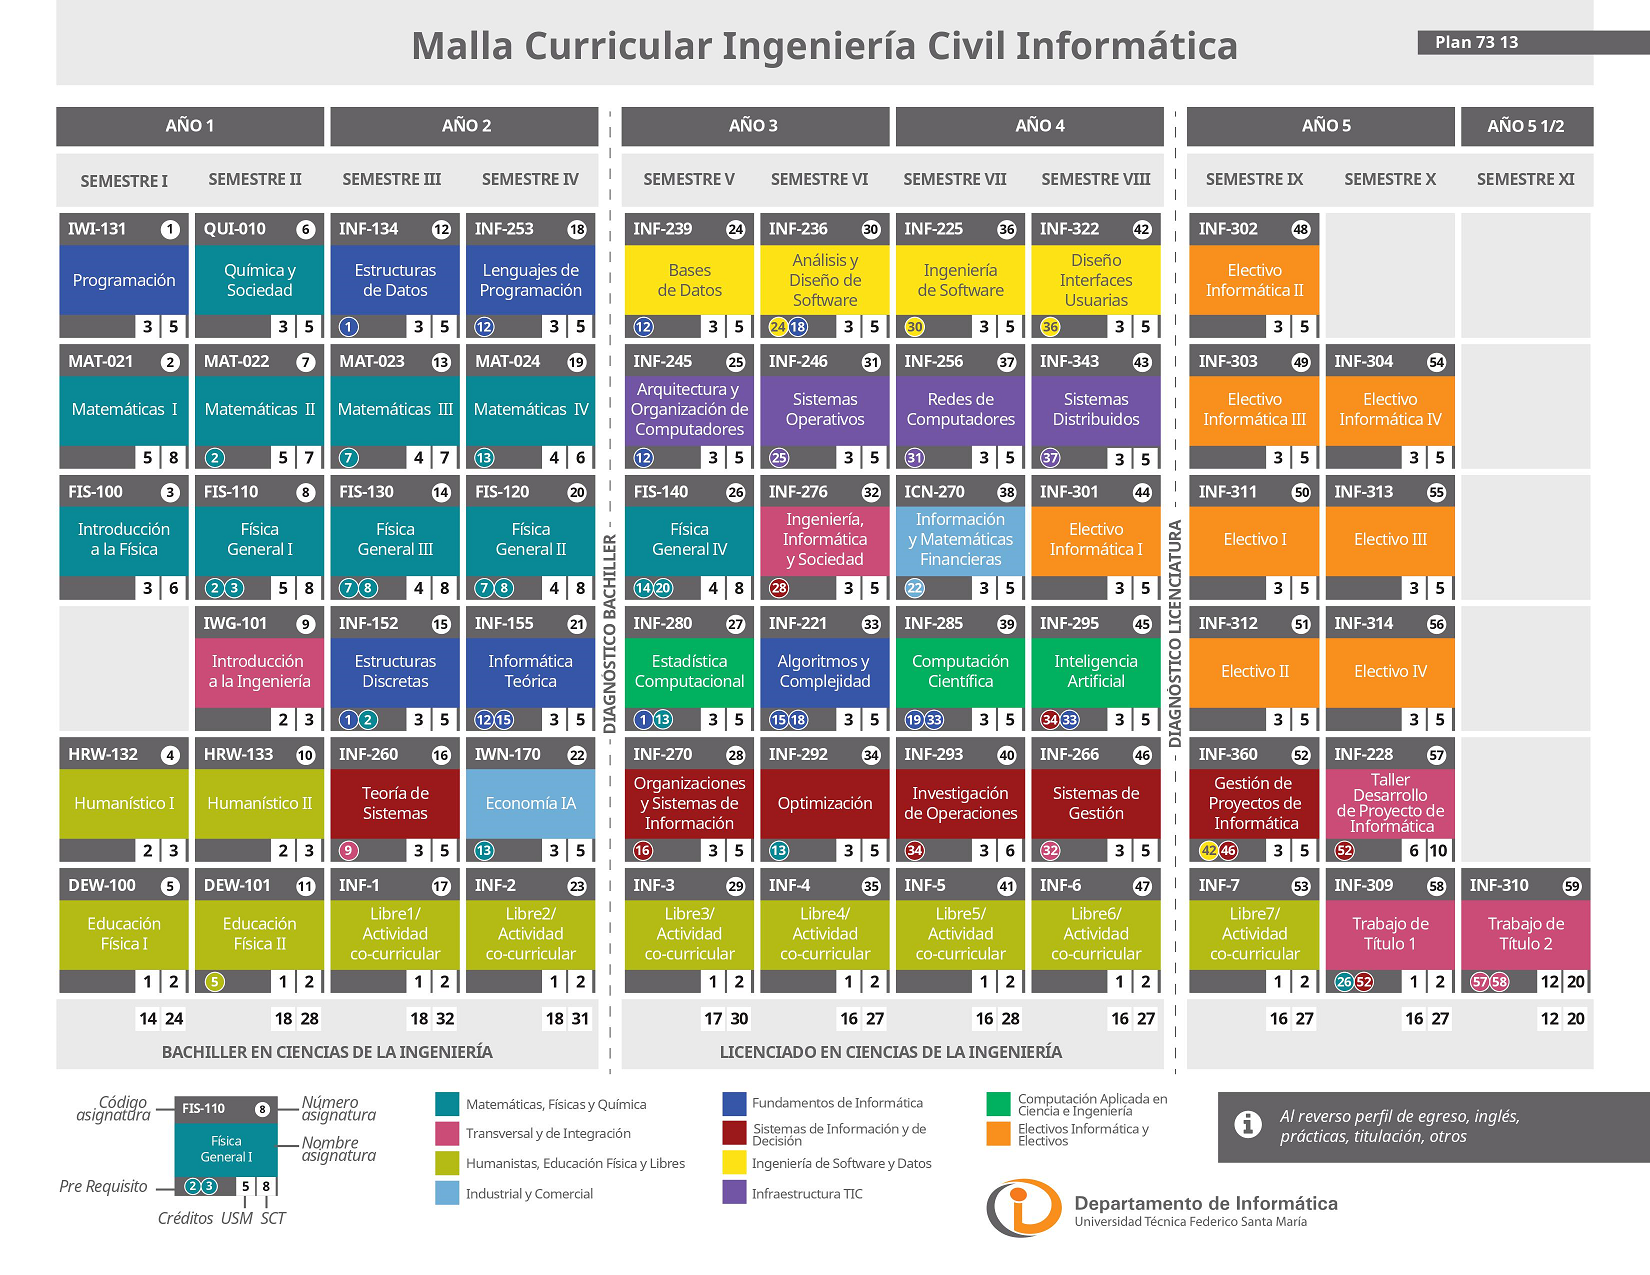
\includegraphics[width=0.8\textwidth]{malla_ingenieria_informatica}
\caption{\label{fig:malla} Malla Curricular Ingeniería Civil Informática.} Fuente: Departamento de Informática.
\end{figure}

%\newpage
%\secnumbersection{VALIDACIÓN DE LA SOLUCIÓN}

Se debe validar la solución propuesta. Esto significa probar o demostrar que la solución propuesta es válida para el entorno donde fue planteada.

Tradicionalmente es una etapa crítica, pues debe comprobarse por algún medio que vuestra propuesta es básicamente válida. En el caso de un desarrollo de software es la construcción y sus pruebas; en el caso de propuestas de modelos, guías o metodologías podrían ser desde la aplicación a un caso real hasta encuestas o entrevistas con especialistas; en el caso de mejoras de procesos u optimizaciones, podría ser comparar la situación actual (previa a la memoria) con la situación final (cuando la memoria está ya implementada) en base a un conjunto cuantitativo de indicadores o criterios.

\subsection{EJEMPLO DE COMO CITAR TABLAS}

Se colocó una tabla que se puede referenciar también desde el texto (Ver tabla \ref{table:coloquios}).

\begin{table}[h]
    \centering
    \caption{\label{table:coloquios} Coloquios del Ciclo de Charlas Informática.} Fuente: Elaboración Propia.
    \begin{tabular}{|p{7cm}|p{7cm}|}
        \hline
        Título Coloquio & Presentador, País \\
        \hline
        ``Sensible, invisible, sometimes tolerant, heterogeneous, decentralized and interoperable... and we still need to assure its quality...''' & Guilherme Horta Travassos, Brasil.\\
        \hline
        ``Dispersed Multiphase Flow Modeling: From Environmental to Industrial Applications''' & Orlando Ayala, EE.UU.\\
        \hline
        ``Líneas de Producto Software Dinámicas para Sistemas atentos el Contexto''' & Rafael Capilla, España.\\
        \hline
        ... & ... \\
        \hline
    \end{tabular}
\end{table}

%\newpage
%\secnumbersection{CONCLUSIONES}

Las Conclusiones son, según algunos especialistas, el aspecto principal de una memoria, ya que reflejan el aprendizaje final del autor del documento. En ellas se tiende a considerar los alcances y limitaciones de la propuesta de solución, establecer de forma simple y directa los resultados, discutir respecto a la validez de los objetivos formulados, identificar las principales contribuciones y aplicaciones del trabajo realizado, así como su impacto o aporte a la organización o a los actores involucrados. Otro aspecto que tiende a incluirse son recomendaciones para quienes se sientan motivados por el tema y deseen profundizarlo, o lineamientos de una futura ampliación del trabajo.

\underline{Todo esto debe sintetizarse en al menos 5 páginas.}


\newpage
\secnumberlesssection{ANEXOS}

En los Anexos se incluye todo aquel material complementario que no es parte del contenido de los capítulos de la memoria, pero que permiten a un lector contar con un contenido adjunto relacionado con el tema.


\newpage
% Bibliografía estilo APA:
\bibliographystyle{apalike-es}
\bibliography{bibliografia}{}

\end{document}
